% Errors

\only<1>{
\centering

$\boxed{\simplicial{u}{G}}$ In the context of graph $G$, node $u$ is simplicial.

\vfill

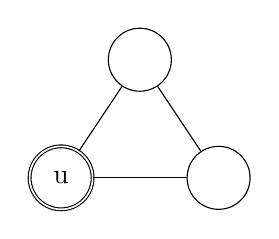
\begin{tikzpicture}
    \node[circle, double, draw, minimum size=8mm] (a) at (0,0) {u};
    \node[circle, draw, minimum size=8mm] (b) at (1,1.5) {};
    \node[circle, draw, minimum size=8mm] (c) at (2,0) {};

    \draw (a) -- (b);
    \draw (a) -- (c);
    \draw (b) -- (c);
\end{tikzpicture}
}

\only<2>{
\[
\inferrule*[Right=SimplicialSingleton]
    {u \not \in V}
    {\simplicial{u}{G+u}}
\]

\vfill

\centering
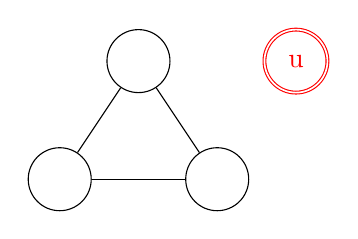
\begin{tikzpicture}
    \node[circle, draw, minimum size=8mm] (a) at (0,0) {};
    \node[circle, draw, minimum size=8mm] (b) at (1,1.5) {};
    \node[circle, draw, minimum size=8mm] (c) at (2,0) {};
    \node[circle, double, draw=red, text=red, minimum size=8mm] at (3,1.5) {u};

    \draw (a) -- (b);
    \draw (a) -- (c);
    \draw (b) -- (c);
\end{tikzpicture}
}

\only<3>{
\[
\inferrule*[Right=SimplicialNode]
    {\simplicial{u}{G}}
    {\simplicial{u}{G + v}}
\]

\vfill

\centering
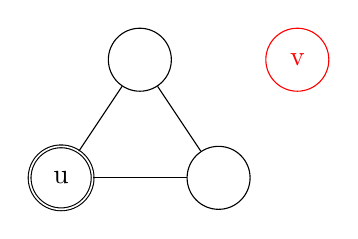
\begin{tikzpicture}
    \node[circle, double, draw, minimum size=8mm] (a) at (0,0) {u};
    \node[circle, draw, minimum size=8mm] (b) at (1,1.5) {};
    \node[circle, draw, minimum size=8mm] (c) at (2,0) {};
    \node[circle, draw=red, text=red, minimum size=8mm] at (3,1.5) {v};

    \draw (a) -- (b);
    \draw (a) -- (c);
    \draw (b) -- (c);
\end{tikzpicture}
}

\only<4>{
\[
\inferrule*[Right=SimplicialEdge]
    {\simplicial{u}{G} \\ u \neq v \\ u \neq w}
    {\simplicial{u}{G + \{ v, w\}}}
\]

\vfill

\centering
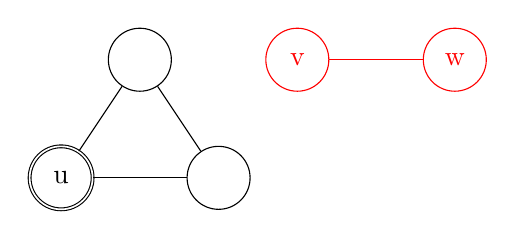
\begin{tikzpicture}
    \node[circle, double, draw, minimum size=8mm] (a) at (0,0) {u};
    \node[circle, draw, minimum size=8mm] (b) at (1,1.5) {};
    \node[circle, draw, minimum size=8mm] (c) at (2,0) {};
    \node[circle, draw=red, text=red, minimum size=8mm] (v) at (3,1.5) {v};
    \node[circle, draw=red, text=red, minimum size=8mm] (w) at (5,1.5) {w};

    \draw (a) -- (b);
    \draw (a) -- (c);
    \draw (b) -- (c);
    \draw[draw=red] (v) -- (w);
\end{tikzpicture}
}

\only<5>{
\[
\inferrule*[Right=SimplicialNeighbor]
    {\simplicial{u}{G}}
    {\simplicial{u}{\addvertex{G}{u}{v}}}
\]

\vfill

\centering
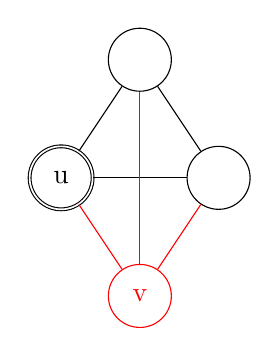
\begin{tikzpicture}
    \node[circle, double, draw, minimum size=8mm] (a) at (0,0) {u};
    \node[circle, draw, minimum size=8mm] (b) at (1,1.5) {};
    \node[circle, draw, minimum size=8mm] (c) at (2,0) {};
    \node[circle, draw=red, text=red, minimum size=8mm] (v) at (1,-1.5) {v};

    \draw (a) -- (b);
    \draw (a) -- (c);
    \draw (b) -- (c);
    \draw[draw=red] (v) -- (a);
    \draw[draw=red] (v) -- (b);
    \draw[draw=red] (v) -- (c);
\end{tikzpicture}
}

% \inferrule*[Right=SimplicialSingleton]
%     {u \not \in V}
%     {\simplicial{u}{G+u}}
% \\
% \inferrule*[Right=SimplicialNode]
%     {\simplicial{u}{G} \\ u \neq v}
%     {\simplicial{u}{G + v}}
% \\
% \inferrule*[Right=SimplicialEdge]
%     {\simplicial{u}{G} \\ u \neq v' \\ u \neq v''}
%     {\simplicial{u}{G + \{ v', v''\}}}
% \\
% \inferrule*[Right=SimplicialNeighbor]
%     {\simplicial{u}{G}}
%     {\simplicial{u}{\addvertex{G}{N(u)}{v}}}


% \only<1>{
% \[
% \renewcommand{\arraystretch}{1}
% \begin{array}{l}
% B_1 := \text{Block (Normal 1) } [] \ [ \\
% \quad r(0) \leftarrow i(0); \\
% ] \ (\text{jump } B_2) \\
% \\
% B_2 := \text{Block (Normal 2) } [ \\
% \quad r(2) \leftarrow \phi[(0, \ \text{Normal 1}); \ (3, \ \text{Normal 2})] \\
% ] \ [ \\
% \quad r(3) \leftarrow r(2) + 1 \\
% ] \ (\text{if } r(3) < 20 \text{ then } B_2 \text{ else } B_3) \\
% \\
% B_3 := \text{Block (Normal 3) } [] \ [] \ (\text{ret } r(6)) \\
% \end{array}
% \]
% }

% \only<2>{
% \[
% \renewcommand{\arraystretch}{1}
% \begin{array}{l}
% B_1 := \text{Block (Normal 1) } [] \ [ \\
% \quad r(\text{RBX}) \leftarrow i(0); \\
% ] \ (\text{jump } B_2) \\
% \\
% B_2 := \text{Block (Normal 2) } [ \\
% \quad r(\text{RBX}) \leftarrow \phi[(\text{RBX}, \ \text{Normal 1}); \ (\text{RBX}, \ \text{Normal 2})] \\
% ] \ [ \\
% \quad r(\text{RBX}) \leftarrow r(\text{RBX}) + 1 \\
% ] \ (\text{if } r(\text{RBX}) < 20 \text{ then } B_2 \text{ else } B_3) \\
% \\
% B_3 := \text{Block (Normal 3) } [] \ [] \ (\text{ret } r(\text{RBX})) \\
% \end{array}
% \]
% }